% !TEX root = ../Thesis.tex


\chapter{Approccio basato sulla self e cross attention}
Usare un approccio basato sulla self e cross attention permette di effettuare la fusione non basandosi su una strategia 
pixel per pixel ma su patch, ovvero 
una piccola regione localizzata o un sottoinsieme di pixel all'interno di 
un'immagine più grande, in genere rettangolare o quadrata. \\\\
L’obiettivo del meccanismo di fusione basato su self e cross attention è combinare 
in modo intelligente più immagini despeckled provenienti da diverse acquisizioni o canali per ottenere un’immagine finale più informativa, pulita e coerente. 
Per affrontare questa problematica, l’approccio proposto in \cite{li2024crossfuse} introduce un meccanismo di fusione basato su self e cross attention, ispirato ai modelli 
transformer, in grado di individuare e valorizzare le componenti informative complementari tra le immagini despeckled, riducendo al contempo la ridondanza residua.
Il paper CrossFuse: A Novel Cross Attention Mechanism based Infrared and Visible Image Fusion Approach mostra che una 
fusione che usa blocchi di self-attention per rinforzare le caratteristiche intra-modalità  
e una cross-attention progettata per esaltare le informazioni non correlate tra le modalità, produce immagini 
fuse con più dettaglio e con meno artefatti, migliorando le strutture rispetto a metodi più semplici. 
Il paper sottolinea inoltre che, in multimodal fusion, la cosa cruciale è valorizzare l’uncorrelation (cioè la complementarità) tra le modalità, 
cosa che la cross-attention è progettata per fare. Questo permette di combinare 
informazioni provenienti da regioni diverse e di differenti modalità, non solo di sommare pixel con pesi locali. 
Il metodo si fonda su una architettura ibrida composta da due blocchi principali.
\subsection{Self-Attention}
La self-attention è un meccanismo introdotto originariamente nei Transformer per consentire a 
una rete di mettere in relazione diverse parti dello stesso input tra loro, pesandole in base alla loro importanza reciproca.
Questo è diverso dalle convoluzioni (CNN) tradizionali, che analizzano solo piccole regioni locali, la self-attention, invece, 
cattura dipendenze globali, anche tra punti molto distanti dell’immagine.
\subsubsection{Funzionamento della Self-Attention}
Sia un'immagine despeckled \(I \in \mathbb{R}^{H \times W \times C}\), dove ogni patch può essere considerato come un \emph{token}.  
Per ogni posizione \(i\) nell'immagine:

\begin{itemize}
    \item \textbf{Query \(Q_i\)}: rappresenta ciò che la posizione \(i\) sta cercando negli altri patch della stessa immagine.
    \item \textbf{Key \(K_j\)}: rappresenta il contenuto informativo della posizione \(j\) rispetto agli altri patch.
    \item \textbf{Value \(V_j\)}: è l'informazione effettiva che la posizione \(j\) può trasmettere a \(i\).
\end{itemize}
Il pixel \(i\) può ``guardare'' altri pixel dell'immagine e decidere quali informazioni (ad esempio strutture, bordi, texture) prendere per migliorare la propria rappresentazione despeckled.

\subsection{Calcolo della Self-Attention}
Il primo passo consiste \cite{vaswani2023attentionneed} nel calcolare la similarità tra ogni Query della target e ogni Key della source, mediante un prodotto scalare:
\[
    \makebox[\textwidth][c]{%
      $\displaystyle
        Q \cdot K^T
      $%
    }
\]
Questo produce una matrice di dimensione $nxm$ in cui $n$ è il numero di elementi della target e $m$ 
quello della source. Ogni entry misura quanto un elemento della target “presta attenzione” a un elemento 
della source. Per stabilizzare la scala dei valori e prevenire problemi numerici, si divide per $\sqrt{d_k}$, ottenendo:
\[
    \makebox[\textwidth][c]{%
      $\displaystyle
        \frac{QK^T}{\sqrt{d_k}}
      $%
    }
\]
Successivamente, applichiamo la funzione softmax riga per riga, trasformando i punteggi in probabilità normalizzate. 
In questo modo, per ogni elemento della target otteniamo un insieme di pesi che indicano quanto ciascun elemento della source contribuisce alla rappresentazione finale:
\[
    \makebox[\textwidth][c]{%
      $\displaystyle
        \alpha = \text{softmax}\left(\frac{QK^T}{\sqrt{d_k}}\right)
      $%
    }
\]
Infine, la matrice dei pesi $\alpha$ viene moltiplicata per la matrice dei Value 
V, combinando le informazioni della source in modo ponderato e producendo i nuovi vettori rappresentativi per la target:
\begin{equation}
    \makebox[\textwidth][c]{%
      $\displaystyle
        \text{Attention}(Q, K, V) = \text{softmax}\left(\frac{Q K^\top}{\sqrt{d_k}}\right)V
      $%
    }
    \label{eq:attention}
    \end{equation}
    
\subsection{Cross-Attention}
La cross-attention \cite{vaswani2023attentionneed} è un meccanismo di attenzione che permette a una sequenza di query provenienti da una sorgente 
(ad esempio un decoder) di pesare gli elementi di un’altra sequenza, da cui provengono le key e le value (ad esempio l’encoder).
In altre parole, essa modella le dipendenze incrociate tra due insiemi distinti di rappresentazioni.
L'attenzione viene calcolata come visto in \ref{eq:attention} con la differenza che nella cross-attention 
le matrici \(Q\), \(K\) e \(V\) provengono da sorgenti diverse. 
\begin{itemize}
  \item \textbf{Query \(Q\)}: proiezione lineare delle rappresentazioni del decoder
  \item \textbf{Key \(K\)}, \textbf{Value \(V\)}: proiezioni lineari delle rappresentazioni del encoder
\end{itemize}
Nel paper CrossFuse: A Novel Cross Attention Mechanism based Infrared and Visible Image Fusion Approach \cite{li2024crossfuse}, 
la cross attention è il cuore del metodo di fusione. Il suo scopo principale non è, come nei transformer 
classici, massimizzare la correlazione tra due insiemi di feature, ma enfatizzare le informazioni complementari 
(cioè non correlate) tra immagini visibile e infrarossa.

\subsection{Architettura del modello}
Due encoder (con la stessa struttura ma parametri diversi) estraggono le feature rispettivamente dall’immagine infrarossa (IR) e visibile (VI), 
servono per catturare le caratteristiche specifiche di ciascuna modalità. Le feature di ciascun encoder passano prima attraverso blocchi di 
self-attention (SA) per migliorare la coerenza intra-modale (dettagli e struttura interna all’immagine).
Poi interviene il Cross-Attention Mechanism (CAM), dove avviene la fusione vera e propria tra le due modalità.
Il decoder ricostruisce l’immagine fusa a partire dalle feature integrate dal CAM, con skip connection per preservare dettagli e salienza.
\subsubsection{Cross-Attention Mechanism}
Il CAM combina self-attention e cross-attention in modo da: potenziare le intra-feature di ciascuna modalità; evidenziare le inter-feature complementari tra IR e VI.
Ogni modalità entra in una catena di blocchi:
\begin{figure}[H]
  \centering
  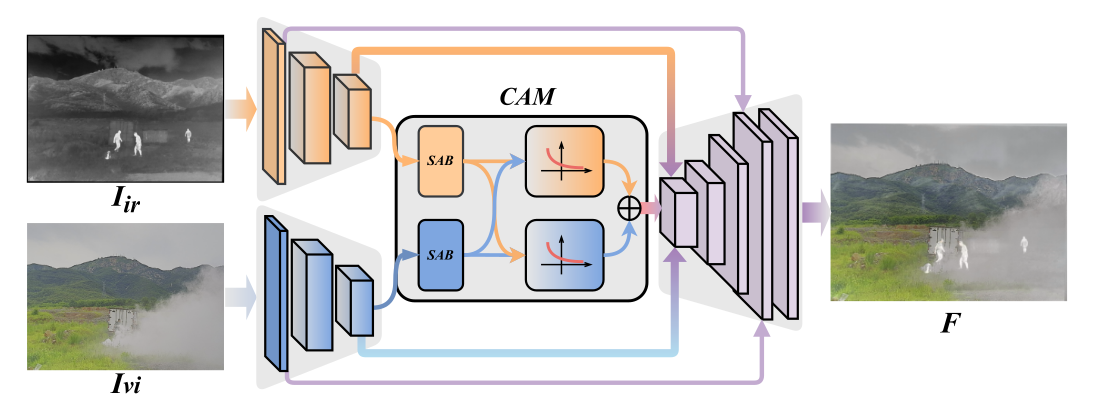
\includegraphics[width=1.0\textwidth]{utils/blocchi.png}
  \caption{I due Encoder hanno la stessa architettura ma parametri differenti. 
  Il meccanismo di cross-attention (CAM) viene utilizzato per fondere le caratteristiche multimodali. 
  “SAB” indica il blocco di self-attention. L’immagine fusa può essere ottenuta tramite il Decoder, 
  che include una connessione lunga proveniente dagli encoder.}
  \label{fig:blocchi}
\end{figure}
I due blocchi di Self-Attention (SA) servono a rafforzare le caratteristiche interne.
L’operazione di Shift/Unshift sposta e ripristina le feature, per aumentare la copertura spaziale globale.
Il Cross-Attention (CA) è il passo cruciale, che integra le due modalità.
\subsubsection{Reversed Softmax}
Il cross-attention è calcolato come nel transformer standard, ma con una differenza fondamentale:
\[
    \makebox[\textwidth][c]{%
      $\displaystyle
        \text{re-softmax(X) = softmax(-X)}
      $%
    }
\]
Questo significa che: invece di dare peso alto alle feature simili (correlate) come fa il softmax classico, 
la re-softmax dà peso alto alle feature dissimili (non correlate). 
CAM enfatizza ciò che una modalità ha e l’altra no, ossia l’informazione complementare, che è essenziale per la fusione

\subsection{Fusione dei modelli}
Nel caso della fusione si hanno quattro autoencoder, ciascuno dedicato a una diversa rappresentazione dell’immagine SAR (SAR-CAM, FANS, SARBM3D, noisy).
Ciò estende il principio di CrossFuse da una fusione bimodale a una 
fusione multimodale. L’idea alla base rimane la stessa: combinare più sorgenti che condividono la stessa struttura spaziale ma presentano contenuti 
informativi parzialmente diversi o complementari, al fine di produrre un’immagine finale più completa, bilanciata e informativa.
Il punto di partenza del sistema è costituito dai quattro encoder, ognuno dei quali apprende a rappresentare la propria modalità secondo il 
suo dominio specifico. Le versioni despeckled prodotte con SARCAM, FANS e BM3D, pur avendo eliminato il rumore di tipo speckle, differiscono 
nel modo in cui trattano i dettagli fini e le strutture deboli: alcune tendono a privilegiare la continuità tonale, altre la preservazione 
dei bordi. L’immagine noisy, invece, pur essendo la più “sporca”, conserva informazione strutturale che spesso viene attenuata durante 
il despeckling. In questo contesto, gli encoder agiscono come estrattori di caratteristiche complementari: ciascuno mappa la propria immagine 
in uno spazio di rappresentazione latente dove si preservano sia i pattern condivisi (ad esempio, i contorni principali) sia le particolarità 
proprie del metodo di despeckling.
Una volta estratte le feature dalle quattro reti, la fusione non può limitarsi a un semplice concatenamento o media ponderata. È qui che 
entra in gioco la cross-attention. Invece di gestire due 
rami (come nel caso infrarosso-visibile), il modello deve essere capace di trattare interazioni multiple, valutando quanto ogni rappresentazione 
contribuisca alla formazione di un contenuto informativo unico. Ogni coppia di modalità può essere posta in relazione attraverso una cross-attention, 
dove la re-softmax viene applicata per enfatizzare la dissimilarità: in questo modo le componenti ridondanti, cioè le parti in cui le 
varie versioni coincidono, vengono attenuate, mentre le parti complementari, presenti solo in uno dei canali, vengono esaltate.
Il passo successivo consiste nel combinare queste diverse mappe di attenzione in una rappresentazione fusa. Questo può essere fatto in modo 
gerarchico, ad esempio con una attention aggregation layer, che raccoglie i risultati delle cross-attention tra le varie coppie di encoder e 
li integra progressivamente. In questo modo si costruisce un’unica mappa di caratteristiche latenti che racchiude i dettagli fini dei vari modelli, 
e riduce al minimo la ridondanza informativa.
Il decoder, a questo punto, ha il compito di ricostruire l’immagine finale partendo da questa rappresentazione fusa. 
\\\\
Il risultato è [DA CAPIRE] 
%un’immagine finale che bilancia la nitidezza e la naturalezza visiva: le aree uniformi appaiono pulite e coerenti, 
%mentre le regioni strutturate, come bordi o pattern, conservano il contrasto e la definizione originaria.
\\\\
Dal punto di vista concettuale, questa architettura si comporta come un “mediatore intelligente” tra diverse visioni dello stesso segnale: non 
sceglie a priori quale metodo di despeckling sia migliore, ma apprende a ponderare dinamicamente l’informazione proveniente da ciascuno in base 
alla sua unicità. La cross-attention, con la re-softmax, garantisce che il modello privilegi la diversità informativa invece della somiglianza, 
rendendo possibile una fusione realmente complementare e non una semplice media delle soluzioni.
